% =====================================================================
\part{The operator studies (Findings 1--4)}
% =====================================================================

\chapter{The kernel-band baseline and its failure (Findings 1--2)}

\section{The operator}
The session's starting production operator: Lin-CDF kernel bands at
$h \in \{0.5, 0.4, 0.3, 0.2\}$, combined by a 4-point Richardson
extrapolation in $h^2$ (``R4''), $\mathrm{NQK} = 16$ Gauss--Legendre
nodes per axis, evaluated at double-double fixed points on a $G = 11$
CDF-uniform grid with a $G_p = 121$ logit-uniform price grid.

\begin{figure}[H]\centering
  
\includegraphics[width=0.9\linewidth]{ov_figs/fig1_richardson_ucurve.png}
  \caption{Richardson order U-curve at the saved R4 fixed point. R4 is
    locally optimal by construction; R3 under-cancels bias and R5
    over-amplifies noise (Vandermonde weight $L^1$-norm doubles per
    added $h$-point). A defensible choice \emph{conditional on the base
    method being right} --- which Finding 1 shows it is not.}
\end{figure}

\section{Finding 1: Richardson does not extrapolate to $h = 0$}
Bandwidths swept from 0.5 down to 0.02 with matched quadrature: the
lookup discrepancy versus \strict{} stays at 0.4--0.6 max-norm. If the
$h^2$ expansion were valid, the error would fall as $h^{2R}$; it does
not, because the level set of the piecewise-linear $P$ has kinks whose
contributions enter at non-integer powers $h^\alpha$ ($\alpha = 1$ or
$3/2$ depending on local geometry). Even-power Richardson cannot
annihilate them.

\begin{figure}[H]\centering
  
\includegraphics[width=0.9\linewidth]{ov_figs/fig3_smallh.png}
  \caption{The smaller-$h$ test: the kernel-band lookup discrepancy vs
    \strict{} does not decay as $h \to 0.02$. The fixed-grid Richardson
    program is unfixable at its root.}
\end{figure}

\textbf{Reconciliation with Part II.} The kernel \emph{is} a consistent
co-area quadrature --- in the \emph{joint} limit $\Delta x \ll h \to 0$.
The failure here is the fixed-grid limit ($h \to 0$ at constant
$\Delta x$): once the band is thinner than the cell size, the
discretized integrand is kinky at the cell scale and the asymptotics in
$h$ break. The two statements are consistent and together they fix the
production rule: \emph{shrink $h$ only together with the grid}.

\section{Finding 2: the deficit collapse under \strict{}}
Re-solving the fixed point under \strict{} co-area + partition-of-unity,
warm-started from R4: the one-to-one deficit collapses by a factor
$\approx 40$ at every cell tested, e.g.\ at $(\gamma, \tau) = (100, 1)$
from $0.255$ to $0.0065$.

\begin{figure}[H]\centering
  
\includegraphics[width=0.9\linewidth]{ov_figs/fig4_strict_vs_R4.png}
  \caption{R4 vs \strict{} fixed points at $(\gamma, \tau) = (100, 1)$:
    the R4 lookup systematically over-predicts the posterior at
    intermediate $p$.}
\end{figure}

\begin{figure}[H]\centering
  
\includegraphics[width=0.9\linewidth]{ov_figs/fig5_mu_curves.png}
  \caption{The lookup at the \strict{} fixed point: smooth, monotone in
    $p$, mirror-symmetric about $p = \tfrac12$.}
\end{figure}

\section{The extended ridge recheck (36 cells)}
The K=3 ``deficit ridge'' (deficit non-monotone in $\tau$ at
intermediate $\gamma$) was re-examined on a $6 \times 6$ $(\gamma, \tau)$
grid under both operators. \textbf{The ridge does not survive}: under
\strict{} the deficit is flat in $\tau$ at $\sim 10^{-2}$, while R4
sweeps from $10^{-9}$ to $10^{-1}$. The operators \emph{cross} near
$\tau \approx 0.4$ --- R4 understates the deficit at low $\tau$
(undersmoothing of smooth cells) and overstates at high $\tau$
(oversmoothing of cuspy cells): a sign-flipping bias, not a uniform one.

\begin{figure}[H]\centering
  
\includegraphics[width=\linewidth]{ridge_figs/slice_per_gamma.png}
  \caption{Deficit vs $\tau$ for $\gamma \in \{1, 10, 30\}$: R4 (red)
    rises steeply; \strict{} (blue) is flat. The crossing near
    $\tau \approx 0.4$ shows the bias flips sign.}
\end{figure}

\begin{figure}[H]\centering
  
\includegraphics[width=0.8\linewidth]{ridge_figs/ratio_per_gamma.png}
  \caption{Collapse factor per cell: up to $\sim 30\times$ at high
    $\tau$, below 1 at low $\tau$.}
\end{figure}

\begin{figure}[H]\centering
  
\includegraphics[width=\linewidth]{ridge_figs/per_cell_bars.png}
  \caption{Per-cell side-by-side deficits across the 18 completed
    low-$\gamma$ cells.}
\end{figure}

\textbf{Important caveat carried forward.} The \strict{} solver itself
is not Lipschitz (the cell-membership flips of Part II); Anderson
reaches $|F| \sim 0.03$--$0.15$ best iterates, not machine-eps fixed
points. The corrected deficit values are best-iterate quantities with
$\sim 10^{-3}$ noise floors. The truly nailed equilibria of the project
live in the consistent-kernel program (\texttt{k3\_coarea\_limit}, joint
central-path limit, $10^{-14}$), and the two views agree on the
qualitative geography: deficit rises with $\tau$, falls with $\gamma$.

\section{Finding 3: robustness $\ne$ correctness (the variant comparator)}
Seven perturbations of the kernel-band lookup --- PCHIP price
interpolation, Neville--Romberg, $\mathrm{NQK} = 24$, $G_p = 241$,
boundary refinements --- agree with each other to $\sim 10^{-5}$ while
\emph{all} sitting 0.05--0.6 from \strict{}. Cross-variant agreement
within an operator family measures conditioning, not truth.

\begin{figure}[H]\centering
  
\includegraphics[width=0.95\linewidth]{ov_figs/fig2_variant_compare.png}
  \caption{The variant comparator: tight cross-variant spread, common
    bias. The defining picture of ``robust but wrong''.}
\end{figure}

\chapter{Alternative lookup builders (Finding 4)}

\section{The field}
Five algorithmically independent builders, evaluated against \strict{}
ground truth at matched fixed points:
\begin{center}\begin{tabularx}{\linewidth}{lXl}\toprule
option & construction & verdict \\
\midrule
A & 3D Chebyshev on CDF-uniform nodes + analytic level-set roots & Runge-divergent; wrong nodes \\
B+ & cube empirical CDF + PCHIP density ratio & \textbf{winner}: median $\sim 10^{-5}$ \\
C & structural ansatz $P = \sigma(\sum_i h(u_i))$ & exact at $\tau \to 0$; Part IV \\
D & adaptive $p$-grid (arclength equidistribution) & $-25\%$ max error, free \\
E & Hermite-cube derivative matching & no improvement \\
\bottomrule\end{tabularx}\end{center}

\begin{figure}[H]\centering
  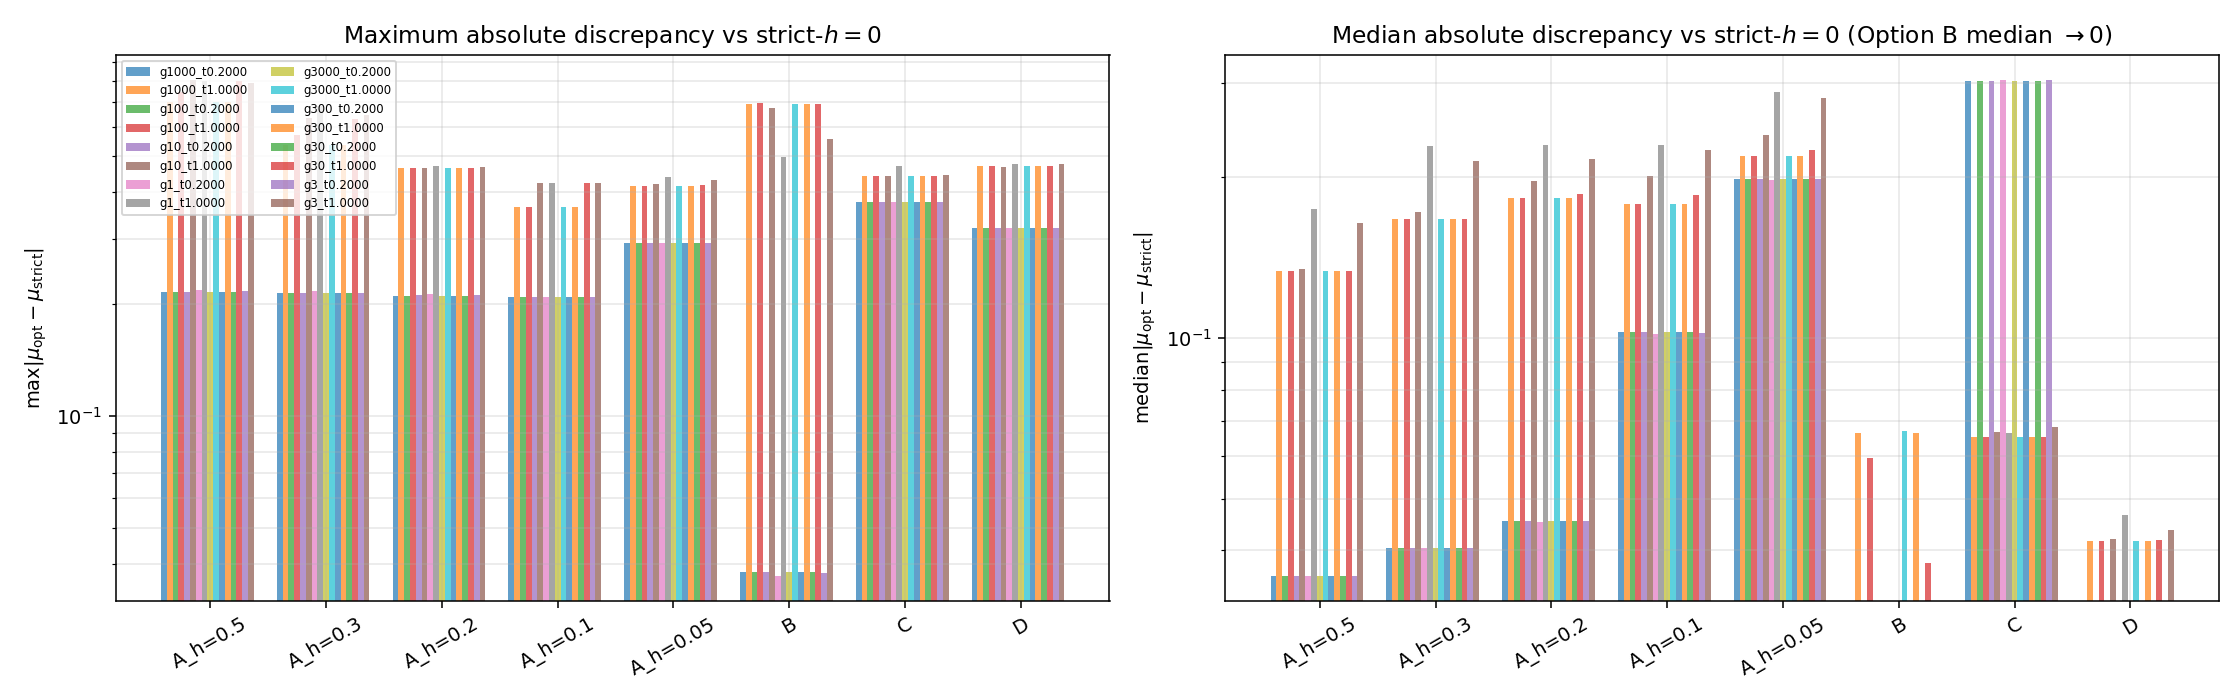
\includegraphics[width=0.95\linewidth]{alts_figs/fig1_max_med.png}
  \caption{Max and median lookup error across builders and
    $(\gamma, \tau)$ cells: Option B+ improves the median by four
    decades over kernel-band R4.}
\end{figure}

\begin{figure}[H]\centering
  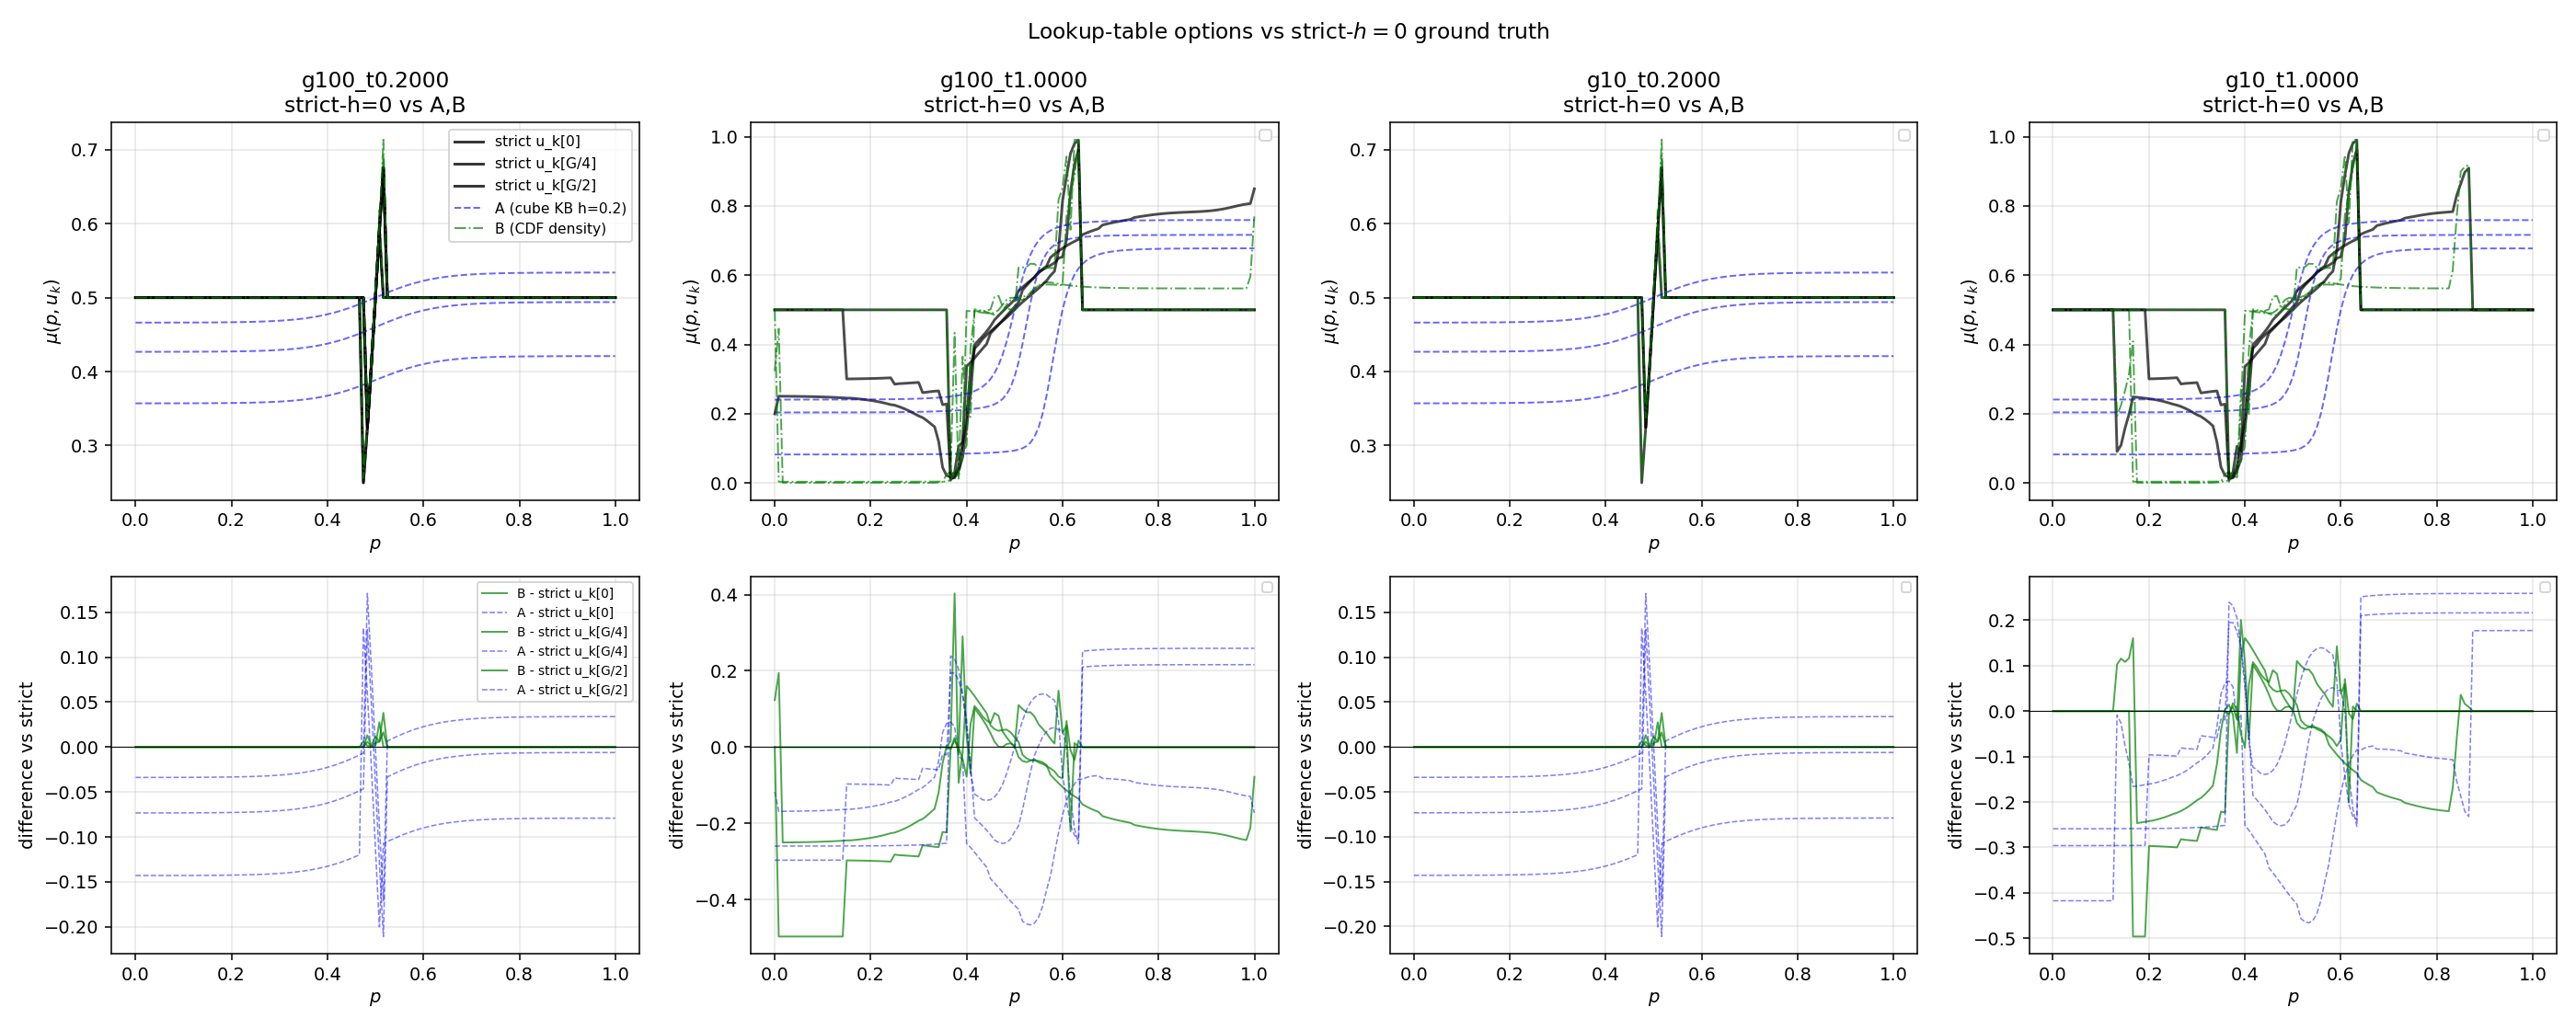
\includegraphics[width=0.95\linewidth]{alts_figs/fig2_mu_curves.png}
  \caption{Visual comparison of the builders' $\mu(p, u_k)$ against
    \strict{}: B+ tracks; A oscillates in the tails; C is exact at
    low $\tau$ but underfits at $\tau = 1$.}
\end{figure}

\section{Option B+ anatomy}
The construction is geometric, not extrapolative: accumulate
Gaussian-weighted cube-cell mass into an empirical CDF in $p$ per state,
differentiate with shape-preserving PCHIP, take the density ratio.
PCHIP's $C^1$-not-$C^\infty$ regularity is exactly matched to the
lookup's cusp structure --- it represents kinks without ringing.

\begin{figure}[H]\centering
  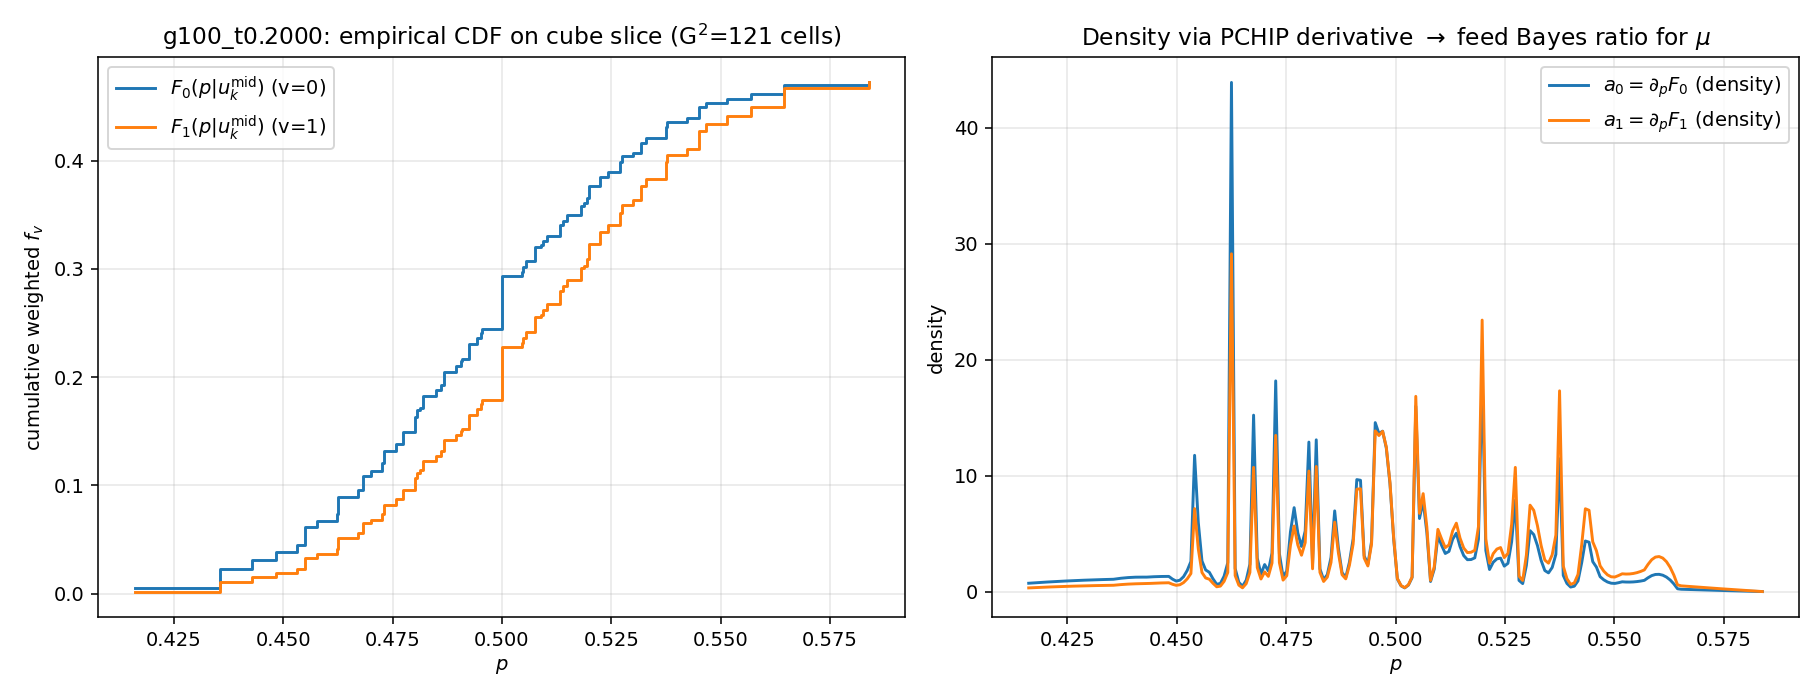
\includegraphics[width=0.95\linewidth]{alts_figs/fig3_cdf_construction.png}
  \caption{Option B+ construction: cube CDF, PCHIP density, resulting
    lookup vs \strict{}.}
\end{figure}

\begin{figure}[H]\centering
  
\includegraphics[width=0.95\linewidth]{optB_figs/fig1_refinement.png}
  \caption{Sub-grid refinement: a $4\times$ refinement inside each bin
    buys roughly a decade of median accuracy at trivial cost (numba).}
\end{figure}

\begin{figure}[H]\centering
  
\includegraphics[width=0.95\linewidth]{optB_figs/fig4_deficit_compare.png}
  \caption{The economic consequence: deficit maps under kernel-band R4
    vs Option B+ over the $(\gamma, \tau)$ region --- the spurious ridge
    versus the true pattern.}
\end{figure}

\textbf{B+ is an evaluator, not a solver.} Used as the inner operator of
a Picard loop it destabilizes the outer iteration --- it lacks the
contraction structure of the co-area operator. The division of labor
that survives to the final recommendation: co-area (kernel or strict)
\emph{solves}; B+/per-segment-Chebyshev \emph{evaluates}.

\section{Option D: the adaptive price grid}
Four monitor functions tested for $p$-grid equidistribution; arclength
of $\mu(p)$ wins (most noise-robust), reduces max interpolation error by
$\sim 25\%$ at $< 5\%$ cost, stacking multiplicatively with B+.

\begin{figure}[H]\centering
  
\includegraphics[width=0.95\linewidth]{optD_figs/fig1_monitor_compare.png}
  \caption{Monitor-function comparison for the adaptive $p$-grid.}
\end{figure}

\begin{figure}[H]\centering
  
\includegraphics[width=0.8\linewidth]{optD_figs/fig3_density.png}
  \caption{Resulting node-density profiles: the arclength monitor puts
    $\sim 23\times$ more nodes where the lookup actually bends.}
\end{figure}

\chapter{The spectral program and its limit}

\section{Chebyshev--Lobatto + analytic contours}
The elegant idea: fit a global 3D Chebyshev polynomial to $P$, then the
level set is an algebraic variety --- companion-matrix root-finding gives
exact contours and the lookup becomes clean 1D quadrature. Two results:
\begin{enumerate}\itemsep2pt
  \item On CDF-uniform nodes the fit diverges (Runge; edge coefficients
        $> 10^6$ at degree 15). Re-solving the FP on true Lobatto nodes
        fixes conditioning ($|F| \sim 10^{-14}$ at $G = 11, 15, 21$).
  \item But convergence of the \emph{lookup} is algebraic only:
        top-edge coefficient $\sim G^{-0.8}$, lookup median
        $\sim G^{-1.6}$. Machine epsilon requires effectively infinite
        $G$. The equilibrium is not analytic at high $\tau$ ---
        consistent with the $C^0$-not-$C^1$ co-area theorem of Part II.
\end{enumerate}

\begin{center}\begin{tabular}{rrrrr}\toprule
$G$ & FP $|F|_\infty$ & top edge coef & lookup max & lookup median \\
\midrule
11 & 6.8e-14 & 0.0491 & 0.434 & 0.251 \\
15 & 2.4e-14 & 0.0198 & 0.407 & 0.127 \\
21 & 4.3e-14 & 0.0110 & 0.380 & 0.081 \\
\bottomrule\end{tabular}\end{center}

\section{Ruling out the operator: the Chebyshev-native fixed point}
To exclude the possibility that the algebraic rate came from mixing the
spectral fit with the kernel-band operator, a Chebyshev-native FP solver
was built (lookup evaluated by analytic contours at the exact cell
price; no kernel, no Richardson, no bilinear interpolation). Same
algebraic decay. \textbf{The slow convergence is a property of the
equilibrium, not of any operator} --- the single most load-bearing
negative result of the spectral program, and the direct motivation for
the \emph{segmented} spectral representation that finally succeeds in
Part V.
